% Typeset with XeTeX
% Allows use of system fonts rather than just LaTeX's ones
% NOTE - if you use TeXShop and Bibdesk (Mac), can complete citations
%  - open your .bib file, type~\citep{xx... and then F5 or Option-Escape
\documentclass[12pt]{article}
\usepackage[margin=1in, letterpaper]{geometry} % set page layout
%\geometry{letterpaper}  % or a4paper
\usepackage[xetex]{graphicx} % allows us to manipulate graphics.
% Replace option [] with pdftex if you don't use Xe(La)TeX
\usepackage{color}
\usepackage[table]{xcolor}
\usepackage{indentfirst}
\usepackage{hyphenat}
\usepackage{epstopdf} % automatic conversion of eps to pdf 
\usepackage{amsmath, amssymb} % Better maths support & more symbols
\usepackage{textcomp} % provide lots of new symbols - see textcomp.pdf
% line spacing: \doublespacing, \onehalfspacing ,\singlespacing
\usepackage{setspace}
\onehalfspacing 
\usepackage{nicefrac}
\usepackage{multirow}
\usepackage{pgfplotstable}
% allows text flowing around figs
% use \begin{wrapfigure}{x}{width} where x = r(ight) or l(eft)
\usepackage{wrapfig}
\usepackage[parfill]{parskip} % don't indent new paragraphs
\usepackage{flafter}  % Don't place figs & tables before their definition 
\usepackage{verbatim} % allows \begin and \end{comment} regions
\usepackage{booktabs} % makes tables look good
\usepackage{bm}  % Define \bm{} to use bold math fonts

% linenumbers in L margin, start & end with \linenumbers \nolinenumbers,
\usepackage{lineno} % use option [modulo] for steps of 5
\usepackage[auth-sc]{authblk} % authors & institutions - see authblk.pdf
%\renewcommand\Authands{ and } % separates the last 2 authors in the list
% control how captions look; here, use small font and indent both margins by 20pt
%{\usepackage[font={sf, footnotesize}]{caption} 

\usepackage[margin=10pt,font={footnotesize,sf}, labelfont=bf, labelsep=endash]{caption}

\setlength{\captionmargin}{20pt}

% don't hyphenate these words (here, helps with table headings)
\hyphenation{homogeneous}
\hyphenation{heterogeneity}

%: FONT
% If you don't want to use system fonts, replace from here to 'Citation style' with \usepackage{Palatino} or similar
%: ************ FANCY FONTS START HERE
\usepackage[no-math]{fontspec} % 'no-math' = keep computer modern for math fonts
\usepackage{xunicode} % needed by XeTeX for handling all the system fonts nicely
\usepackage[no-sscript]{xltxtra} 
\setmonofont[Scale=0.8]{PT Serif} % typeface for \tt commands
\setsansfont{Avenir} 
\defaultfontfeatures{Mapping=tex-text}
\setmainfont{Minion Pro}
%\setmainfont{Source Sans Pro}
%: ************ FANCY FONTS END HERE

%:CITATION STYLE
% natbib package: square,curly, angle(brackets)
% colon (default), comma (to separate multiple citations)
% authoryear (default),numbers (citations style)
% super (for superscripted numerical citations, as in Nature)
% sort (orders multiple cites into order of appearance in ref list, or year if authoryear)
% sort&compress: as sort, + multiple citations compressed (as 3-6, 15)
\usepackage[numbers,comma,sort&compress]{natbib}
\usepackage{breakcites} % allows long cite lists to be broken over lines (better formatting)
% Numbering style in bibliography (this may be over-ruled by another .sty package)
% (e.g, here it will be 1. and not [1] as in standard LaTeX)
\makeatletter
\renewcommand\@biblabel[1]{#1.}
\makeatother




%:SHORTCUT COMMANDS
% Maths
\newcommand{\ddt}[1]{\ensuremath{\frac{{\rm d}#1}{{\rm d}t}}}  % d/dt
\newcommand{\dd}[2]{\ensuremath{\frac{{\rm d}#1}{{\rm d}#2}}} % dy by dx  - \dd{y}{x}
\newcommand{\ddsq}[2]{\ensuremath{\frac{{\rm d}^2#1}{{\rm d}#2^2}}} % second deriv
\newcommand{\pp}[2]{\ensuremath{\frac{\partial #1}{\partial #2}}} % partial \pp{y}{x}
\newcommand{\ppsq}[2]{\ensuremath{\frac{\partial^2 #1}{\partial {#2}^2}}}
\newcommand{\superscript}[1]{\ensuremath{^{\textrm{#1}}}} %normal (non-math) font for super/subscripts in text
\newcommand{\subscript}[1]{\ensuremath{_{\textrm{#1}}}}
\newcommand{\positive}{\ensuremath{^+}}
\newcommand{\negative}{\ensuremath{^-}}
% Editing
\newcommand{\red}[1]{{\color{red}{#1}}}
\newcommand{\redtext}[1]{{\color{red}{#1}}}
\newcommand{\blue}[1]{{\color{blue}{#1}}}
\newcommand{\bluetext}[1]{{\color{blue}{#1}}}
\newcommand{\scinot}[2]{\ensuremath{#1 \times 10^{#2}}}
% Standard stuff
\newcommand{\be}{\begin{equation}}
\newcommand{\ee}{\end{equation}}
\newcommand{\bea}{\begin{eqnarray}}
\newcommand{\eea}{\end{eqnarray}}
\newcommand{\ie}{\textit{i.e.}}
\newcommand{\etal}{\textit{et al.}}
\newcommand{\khi}{Ki67$^\text{hi}$}
\newcommand{\klo}{Ki67$^\text{lo}$}
\newcommand{\looic}{$\Delta$LOO-IC}



%:Title, authors and institutions
\title{Complete and repeated replenishment of the follicular B cell compartment \red{ GC too!} ensures repertoire diversity throughout life}
\author[1]{Melissa Verheijen}
\author[2]{Sanket Rane}
\author[1]{Andrew J. Yates}
\author[1]{Benedict Seddon}
\affil[1]{\small  Institute of Immunity and Transplantation, Division of Infection and Immunity, UCL,  Royal Free Hospital, Rowland Hill Street, London NW3 2PF, United Kingdom}
\affil[2]{Department of Pathology and Cell Biology,  Columbia University Medical Center, 701 West 168th Street, New York, NY 10032, USA}
\date{{\small Address correspondence to either author; {\small \tt benedict.seddon@ucl.ac.uk, andrew.yates@columbia.edu}}\\
{\small Running title: Complete turnover of naive B cells}\\
{\small Keywords: B cells, mathematical modelling}}
%%%%%%%%%%%%%%%%%%%%%%%%%%
\begin{document}
\maketitle

\linenumbers
%\subsubsection*{Summary}
%Generating and maintaining a diverse repertoire of naive T cells is essential for protection against pathogens, and developing a mechanistic and quantitative description of the processes involved lies at the heart of our understanding of vertebrate immunity. Here we review the biology of naive T cells from birth to maturity and outline how the integration of mathematical models and experiments has helped us to develop a fuller picture of their life-histories.

\section*{Introduction}
B cells v important etc. Develop in bone marrow, where Bcr genes undergo rearrangement. Cells that successfully express a mature BCR migrate to the spleen where they enter a transitional pool of cell, characterised by CD93 expression, and complete development (ref). New B cells enter the spleen and first upregulate CD23 followed by downregulation of IgM. These markers together identify three stages of transitional cell maturation. During the T1 stage, B cells with autoreactive BCRs undergo negative selection. During the T2 stage, cells commit to either a follicular B cell fate, progressing through the T3 stage or are diverted to develop into marginal zone B cells, losing expression of CD23, upregulating IgM and expressing CD21.
Survival of mature B cells is dependent upon BAFFR and BCR signalling. Blockade of BAFF in vivo results in a rapid loss of mature B cells, while BAFFR-/- mice undergo normal BM development and generation of transitional populations, but fail to accumulate mature follicular or marginal Z B cells. Similarly, signals from the BCR are critical for B cell survival. Ablation of BCR expression by  mature B cells results in their rapid loss~\citep{Lam:1997ve}. Expression of Syk, that transmits signals from the BCR, is also required for long term survival of both follicular and MZ B cells~\citep{Schweighoffer:2013jx,Konigsberger:2015gl}.

While it is clear that establishment of the B cell pool relies upon \textit{de novo} generation of B cells in the bone marrow, it is less clear how the stable B cell compartment is maintained in the steady state through out life. B cells have been reported to undergo homeostatic proliferation in lymphopenia~\citep{MeyerBahlburg:2008bc, Cabatingan:2002fm} and there is also evidence of quorom sensing in controlling the overall size of the B cell compartment (Freitas refs). However, it is not known what the relative contribution of self renewal and bone marrow development play in maintaining the compartment. Much of our understanding B cell homeostasis in the steady state comes from analysing BrDu DNA label incorporation. Developing B cells undergo extensive expansion as pre-B cells prior to BCR rearrangement, but remain quiescent and non cycling thereafter  as they develop through transitional stages~\citep{Srivastava:2005jja}. Thus, monitoring the kinetics with which new BrdU labelled cells emerge and are incorporated into the mature pool provides information about B cell life spans and pool maintenance. Such studies reveal that the bone marrow does make substantial daily contribution to the mature follicular pool, estimated at \scinot{3.8}{5} cells a day. Early studies suggest that turnover in B cells in adult mice is slow, with only around half the pool replenished over a 12 week period, and that labelled cells incorporate in a non-linear manner, reaching a plateau over this time period~\citep{Forster:1990tl, Fulcher:1997dr}. 

Blocking B cell development by interfering with IL-7 signalling suggests that mature B cells can persist for weeks to months~\citep{Grabstein:1993jb}. Similarly, inducible deletion of Rag2 results in loss of B cell production, and similar estimates of B cell life span, with 90\% of cells lost within 4 months~\citep{comp:2001ti}. Resource competition is thought to limit the overall size of the B cell compartment. The numbers of B cells found in parabiosed WT pairs vs Rag2\superscript{-/-} and WT mice is the same, despite the latter mice having half the output of new B cells from the bone marrow~\citep{Agenes:1997hk}. There is also the view that the peripheral B cell pool is heterogeneous \red{isn't this unsurprising since there are multiple subsets?}, containing both short lived and long lived populations, although this likely reflected immature and mature populations~\citep{Fulcher:1997dr}.

Despite this extent of study, we still lack understanding of how B cell compartments are maintained throughout the life course. BrdU labelling studies are necessarily limited in duration, due to analogue toxicity in the longer term. Similarly, use of irradiated chimeras to monitor dynamics of repopulation and maintenance are complicated by the lymphopenic environment that induces transitional cells to undergo homeostatic proliferation~\citep{MeyerBahlburg:2008bc}. To address these issues, we employed the method of temporal fate mapping (hogan cite) to measure the contribution and extent of tonic reconstitutions of B cell compartments from the bone marrow. We then tested different models of B cell maintenance to find the most parsimonious explanation for the dynamics during life. 

\clearpage
\section*{Results}
\subsection*{Busulfan treatment permits reconstitution of bone marrow HSC niche without perturbing peripheral mature B cell compartments}
%figure 1 model validation
In order to determine the rules governing the maintenance of peripheral follicular mature (FM) B cell pools, and assess the contribution of de novo B cell development to this , we analysed B cell compartments using a previously published method of temporal fate mapping~\citep{Hogan:2015bd}. Briefly, in this approach, treatment of mice with the conditioning drug, busulfan, ablates the host haematopoetic stem cell (HSC) compartment but leaves mature peripheral haematopoetic compartments unaffected. The depleted HSC niche is then specifically reconstituted with congenically labelled HSC progenitors. Although host HSC replacement is rarely complete, levels of 80-95\% replacement with donor  HSC are typical, and measuring the emergence of donor derived cells serves as an accurate proxy for new cell development from the time of BMT. \red{Do we need to say this? i feel it makes us look more approximate than we are... as long as we normalise to the BM or transitionals, it doesn't matter what chimerism we achieve!}  The infiltration and replacement of mature peripheral haematopoetic compartments by the progeny of donor HSC can then be followed for the remainder of the hosts life (Figure~\ref{fig:Model_validation}A). 
%fig 1A - busulfan model

\begin{figure}[htbp] %  figure placement: here, top, bottom, or page
   \centering
%   \includegraphics[width=\linewidth]{Figure.pdf} 
   \caption{(A) Busulfan model cartoon (B) scatters of cell no. vs age in chimeras vs WT in T1, MZ, FM and GC populations - and perhaps a summary of Ki67 too (C) gating for B220 vs AA4.1, LgM vs CD23, donor vs host - then show \% donor in T1 vs time post BMT }
   \label{fig:Model_validation}
\end{figure}


To analyse the maintenance of FM B cells by temporal fate mapping, we generated chimeras by treatment of CD45.1 C57Bl6/J hosts with busulfan followed by their reconstitution with T and B depleted bone marrow from CD45.2 C57Bl6/J donors. We have previously confirmed that busulfan treatment has no detectable impact upon the long-term survival, proliferation or maintenance of peripheral T cell compartments~\citep{Gossel:2017iu,Hogan:2015bd}. However, to confirm that the same was also true for mature B cell compartments, we compared absolute numbers and expression of Ki67 amongst peripheral B cells at different times following busulfan treatment  and  reconstitution.  As compared with untreated, age matched controls, we observed no significant effects upon either cell numbers or Ki67 levels amongst either transitional, FM or GC B cells (Figure~\ref{fig:Model_validation}B).
%fig 1B - scatters of cell no. vs age in chimeras vs WT in T1, MZ, FM and GC populations - and perhaps a summery of Ki67 too ? 

In order to use emergence of donor B cells as a proxy for total new B cell development since BMT, 
%\red{again, I don't think this is what we are doing. We never need to say that all new cells are donor-derived. it's just that the donor cells are a constant proportion of the new cells}  
we require knowledge of donor/host chimerism in HSC or B cell progenitor pools. Measuring chimerism in B cell progenitors of bone marrow from different bones revealed subtle variations between sites (Figure~S1). Such variations in chimerism were not observed amongst mature B cell populations in individually processed lymph nodes, so did not represent simple technical variation (Figure~S1). This most likely reflects variation in the extent of drug mediated HSC ablation, perhaps due to stochastic variation in drug penetrance of different bones. Therefore, chimerism in no single bone marrow site can be representative of total bone marrow output. Although B cell development is initiated in the bone marrow,  developing B cells must migrate to the spleen to continue development as AA4.1\superscript{+} transitional B cells \red{(ref)}. In particular, AA4.1\superscript{+} IgM\superscript{hi} CD23\superscript{lo} transitional 1 (T1) subset is an obligate, splenic stage, that the vast majority of bone marrow derived B cells  transit.  Therefore, the donor/host composition of T1 cells represents an aggregate of immediate bone marrow output from all the anatomically distinct sites of haematopoesis at any given time. Consistent with this,  donor chimerism in T1 compartment of chimeras revealed a rapid switch from host to donor origin cells following BMT, reaching levels between \red{X and Y\% }(Figure~\ref{fig:Model_validation}C). Importantly, the extent of donor chimerism remained similar in chimeras over time, suggesting that chimerism, once established, was stable, consistent with previous studies~\citep{Hogan:2015bd}. Therefore, we used donor chimerism in the T1 compartment as a proxy for \textit{de novo} B cell development since BMT. %Normalising donor chimerism in downstream compartments to the 
%fig S1 - % donor in different bones
%fig 1C gating for B220 vs AA4.1, LgM vs CD23, donor vs host - then show % donor in T1 vs time post BMT

\red{I think we need to reframe things hereon a bit, putting FM and GC on more of an equal footing. In particular the Ki67 section (below this one) refers to FM only}

\subsection*{Temporal fate mapping reveals complete replacement of follicular mature pool by HSC progeny}
%figure 2 
We next analysed donor reconstitution amongst CD23\superscript{hi} transitional 2/3 (T2/3) and FM B cells in chimeras. There was a high degree of correlation in donor chimerism observed in these populations in LN, spleen and bone marrow in easch mouse (Figure~\ref{fig:Raw_FMplots}A), confirming that these  mature B cell populations are freely recirculating between the different lymphoid sites. The kinetics of donor chimerism in these populations revealed rapid replacement of T2/3 cells and more progressive replacement of FM B cells (Figure~\ref{fig:Raw_FMplots}B). To visualise the extent of replacement since BMT, we normalised the donor chimerism in these more mature compartments to the donor chimierism among T1 splenocytes from the same individual, which we used a proxy for the donor:host composition of newly-generated bone marrow derived B cells. This normalisation allows us to visualise the proportion of each compartment that has been replaced over time, since complete turnover is reached when the chimerism of the downstream compartment equals that of T1 cells. This procedure also allows us to control for normal variation in the level of stable bone marrow chimerism achieved across mice. As anticipated, the T2/3 compartment underwent complete and rapid replacement within \red{X} weeks following BMT (Figure~\ref{fig:Raw_FMplots}C). The kinetic of replacement of T2/3 cells in LN slightly lagged that in the spleen, likely reflects the timing involved in differentiation of T1 to T2 and the onset of recirculation and T2 cells populating LN. Strikingly, FM B cells underwent almost complete replacement by 20 weeks following BMT. \red{We should put GC in here too....?}

%2A scatters of % donor in matFM in bm vs spn vs ln
%2B - scatters of raw % donor in T2/3 and FM vs time post BMT
%2C - scatters of FracNew in T2/3 and FM

\begin{figure}[htbp] %  figure placement: here, top, bottom, or page
   \centering
%   \includegraphics[width=\linewidth]{Figure.pdf} 
   \caption{(A) scatters of \% donor in matFM in bm vs spn vs ln (B) scatters of raw \% donor in T2/3 and FM vs time post BMT (C) scatters of FracNew in T2/3 and FM }
   \label{fig:Raw_FMplots}
\end{figure}





\subsection*{Ki67 protein levels in developing B cells serve both as a reporter of recent cell division and as a molecular clock}
% Figure 3 - (A) ki67 levels in BM, T1, T2, T3, FM 
% (B) Ki67 frequencies amongst donor and host post BMT
The kinetics with which new (donor-derived) B cells percolate into peripheral B cell subsets and displace older host-derived cells allow us to map B cell differentiation pathways,  quantify the homeostatic dynamics of each subset, and establish their rules of replacement.
%The kinetic of infiltration of donor cells into the FM compartments is rich in information concerning the mechanisms governing the long term maintenance of the pool.
The shifting donor/host composition of FM B cells in chimeras distinguishes cells of different ages, developing either before or after BMT, and is a window into homeostatic mechanisms that may conceal heterogeneity in turnover and/or potentially time-varying rates of loss or proliferative renewal. We also generated chimeras using hosts of varying ages, to help us evaluate any influence of host age on B cell maintenance. 
	

In order to investigate candidate models of B cell maintenance, we encoded different candidate mechanisms as mathematical models and compared the ability of these models to describe the data. 
%data using different mechanistic models of B cell maintenance, to see which could best describe the dynamics of the FM B cell compartment throughout life.
To help distinguish the contributions of death and proliferation, we measured Ki67 levels in different compartments of chimeras as a marker of recent cell division. In T cells, Ki67 expression is induced at G1 stage of cell cycle, prior to cell division, but persists for more than three days after cell division has ended~\citep{Gossel:2017iu,Hogan:2013id}. 

Analysis of Ki67 expression revealed variation across stages of B cell development in bone marrow, transitional stages and mature FM B cells (Figure~\ref{fig:Ki67}A). Pre-B cells undergo extensive proliferation during development, and exhibit a high, unimodel distribution of Ki67 expression. In contrast, transitional populations in the spleen do not undergo cell division as they mature~\citep{Srivastava:2005jja}. However, Ki67 levels were also high in these populations, while only a small subset of FM B cells were found to express Ki67 (Figure~\ref{fig:Ki67}A). Following BrdU administration, labelled T2 cells are detected in the spleen within 2 days~\citep{Srivastava:2005jja}, suggesting that the time between cessation of cell division of progenitors in the bone marrow and the development of their progeny can be as little as 2 days, far shorter than the 3-4 day lifetime of Ki67 protein suggested by T cell studies. Therefore, it is most likely that Ki67 expression measured in transitional populations does not represent active cell division, but is rather inherited from  cell division events amongst precursors in the bone marrow. Consistent with this view, Ki67 levels in transitional populations remained unimodal in distribution but exhibited a progressive fall in median level as cells matured through the transitional stages and entered the mature FM compartment (Figure~\ref{fig:Ki67}A) \red{NICE}. In FM B cells, a smaller subset of cells expressed Ki67. While this may indicate cell division of mature cells, contributing to the maintenance of the pool, some expression also represent residual Ki67 protein present in newly generated B cells. Consistent with such a possibility, analysing Ki67 expression in donor and host cells revealed much higher Ki67 levels amongst donor origin cells, that reduced with time after BMT, to eventually match levels observed in host cells (Figure~\ref{fig:Ki67}B). In light of this, models were formulated in which Ki67 is explained by both the influx of {\khi} progenitors and de novo cell division amongst mature FM B cells. 

	
	

%: Figure - Ki67 host donor
\begin{figure}[htbp] %  figure placement: here, top, bottom, or page
   \centering
%   \includegraphics[width=\linewidth]{Figure.pdf} 
   \caption{(A) ki67 levels in BM, T1, T2, T3, FM (B) Ki67 frequencies amongst donor and host post BMT }
   \label{fig:Ki67}
\end{figure}




%The kinetics with which new (donor-derived) B cells percolate into peripheral B cell subsets and displace older host-derived cels allow us to map their differentiation pathways, quantify their homeostatic dynamics, and determine the rules of replacement within each subset.
	


%The busulfan chimera system allows us to t fate of newly made B cells as they develop and differentiate into mature subsets.

	
	
\subsection*{Follicular Mature B cells are a homogeneous, slowly dividing population whose lifespan increases with age}

%We generated timecourses of numbers and Ki67 expression levels of host and donor cells within the FM B cell pool in mice after the establishment of stable bone marrow chimerism in mice. To allow us to examine any impact of age on homeostatic dynamics, we generated chimerism in mice of ages spanning ?? and ??? weeks, and followed them out to a year of age. 	We wanted to use this information to	 assess the relative support for a variety of different models of FM B cell homeostasis, shown schematically in Figure~\ref{fig:FM-model-sketches}. 

To quantify the dynamics of FM B cell development and homeostasis, we used mathematical models to describe the kinetics with which donor-derived B cells percolate into mature B cell subsets identify
 
We used mathematical models to describe the timecourses of the numbers and Ki67 expression levels of   host and donor cells within the FM B cell pool in mice after the establishment of stable bone marrow chimerism allowed us assess the relative support for a variety of different models of FM B cell homeostasis, shown schematically in Figure~\ref{fig:FM-model-sketches}. 

We assumed that FM cells circulate freely in the lymphatic system \red{CITE} and \red{\bf  indeed found no differences in the levels of Ki67 expression or kinetics of development of donor:host chimerism in FM cells in spleen and lymph nodes (SI figures)} \blue{Though this recaps Fig 2 to a degree}   and so we pooled the numbers of these cells recovered from spleen and lymph nodes when modelling their dynamics.



	
In all models, newly-differentiated FM B cells are generated at a rate proportional to the size of their precursor population, which  could be either T1, T2, or T1 and T2 combined. The simplest model (Figure~\ref{fig:FM-model-sketches}A)  assumed that  FM B cells, whether host or donor, are generated from their precursors at the same constant rate, and form a homogeneous population which undergoes turnover (loss) and self-renews through division at constant rates. This model predicts a smooth, continuous approach to stable chimerism in the FM B cell pool. 
%However the approach to stable chimerism appeared to initially be rapid and then gradually slow (Figure~\ref{fig:results_FM}B).
However, the precise shape of this curve is rich in information regarding the processes of influx, loss and self-renewal. To detect and explain any more complex homeostatic dynamics, we considered three extensions to this basic model. In the first, the rate of turnover or division might vary with host age (the `time dependent' model, Figure~\ref{fig:FM-model-sketches}B). In the second, the FM pool is homogeneous with constant rates of division and turnover, but fed from the source population at a rate that changes with age  (Figure~\ref{fig:FM-model-sketches}C).  In the third extension,  FM B cells comprise two independent subpopulations turning over at different rates (Figure~\ref{fig:FM-model-sketches}D). In this scenario the donor chimerism will initially increase rapidly as the subpopulation with faster turnover is replaced, followed by a more gradual approach to stable chimerism as the more persistent subpopulation, with slower turnover, is replaced. 

%: Figure - model sketches
	\begin{figure}[htbp] %  figure placement: here, top, bottom, or page
	   \centering
	   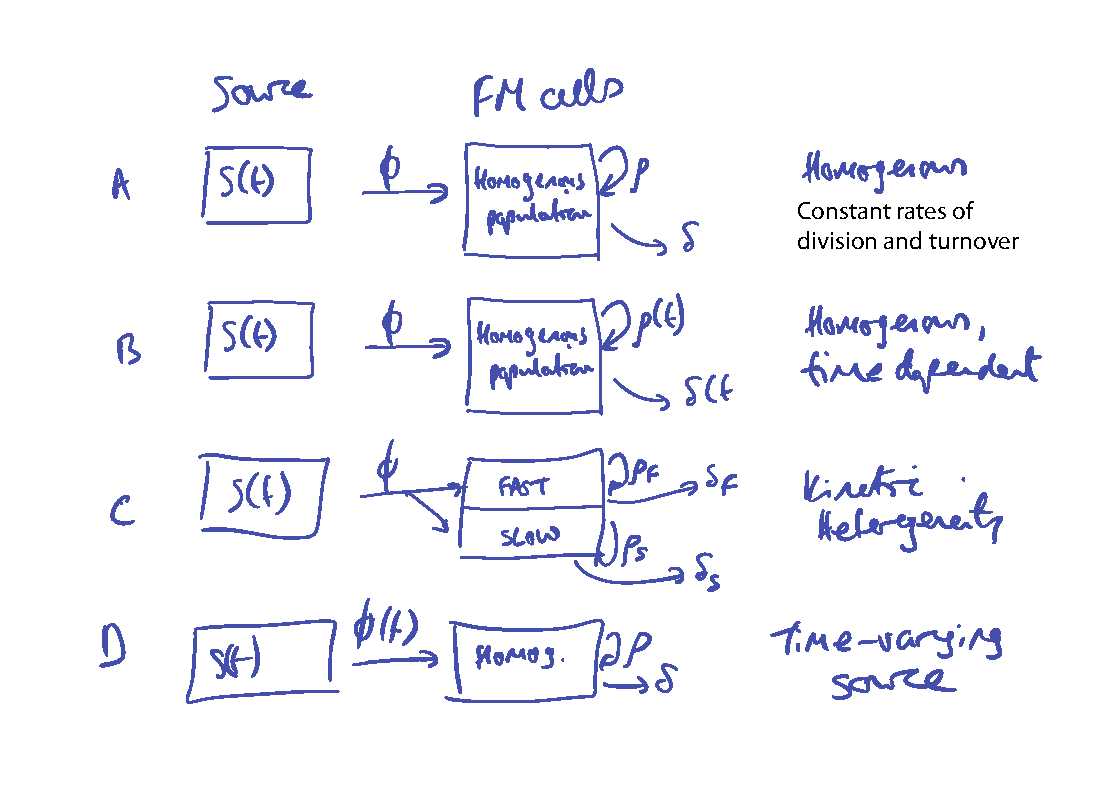
\includegraphics[width=0.8\linewidth]{figures/FM-Model-Sketches.pdf} 
	   \caption{Schematic descriptions of the candidate models of FM B cell homeostasis}
	   \label{fig:FM-model-sketches}
	\end{figure}


%It is an upper bound because there may be continued immigration of YFP-expressing cells labelled earlier in development; for FM B cells, which we assume derive from the rapidly-turning o




	
%\red{I think should drop incumbent. No signal in data to support trying it?}
%An alternative explanation of this time-varying kinetic is that the FM pool comprises independent sub-populations with different but constant rates of division and turnover, each fed from the T1 source.  In this scenario, less persistent populations (those with a high net loss rate $\lambda$) will be replaced most rapidly after BMT, giving an initial steep upslope in chimerism. There will then follow a slower increase as the more persistent FM subpopulations (with low $\lambda$) are replaced by donor cells relatively slowly.
We fitted each model  simultaneously to the timecourses of (i) the numbers of FM B cells, (ii) the chimerism within FM B cells normalised to that in T1 (the earliest common precursor to all populations considered), and (iii) the proportions of host and donor FM B cells expressing Ki67. To help discriminate between these models, we made use of observations from  Ki67-CreER-YFP reporter mice.  We measured  the frequencies of YFP-expressing FM B cells   15 and 66d after the  induction of YFP expression in cells expressing Ki67 during tamoxifen treatment\red{(Figure)}.  The rate of decline in YFP expression  is an upper bound on the net rate of loss of FM B cells (death minus division). We used a Bayesian inference method to incorporate this information into the fitting process (see Methods). 
\red{I feel like this needs a bit more clarification}

We found strongest support for the model in which the turnover rate  changes with host age and the division rate remains constant, with T1 transitional cells as the direct precursor of FM B cells.  Fits and data are shown in Fig.~\ref{fig:results_FM}; see Methods for the mathematical formulation of the models and the fitting strategy.  The measures of relative support for this and the alternative models are given in Table~\ref{tab:FM-AICs}.

%: Figure - FM results

 	\begin{figure}[htbp]
		\centerline{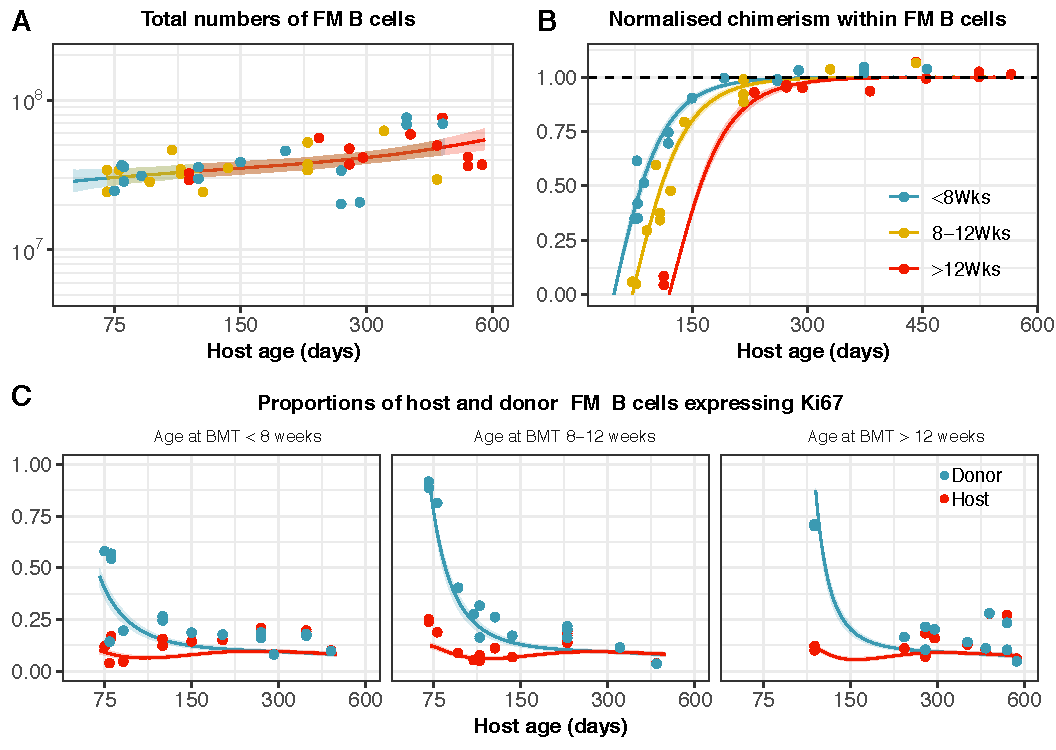
\includegraphics[scale = 0.85] {Results_FM_T1.pdf}}
		\caption{ \textbf{Population dynamics of FM B cells in busulfan chimeric mice}, using the best-fitting model in which cells divide at a constant rate and their mean lifespan increases with host age.
		%The model was fitted simultaneously to the extended timecourses of total cell counts of FM B cells pooled from LN and spleen in busulfan chimeras, the donor fractions in FM B cells normalised to the chimerism in T1 cells and the proportion of cells that were \khi\ within host and donor FM B cells.
		Solid lines denote the most probable simultaneous description of the observations of (A) cell counts, (B) the  chimerism within FB cells normalised to that in T1,  and (C) the proportions of host and donor cells expressing Ki67. Shaded envelopes indicate the effect of uncertainty in parameters on the model fit, generated by drawing samples from the posterior distribution of parameter estimates and shading within the 4.5 and 95.5 percentiles of the resulting model predictions. Different colours in (A) and (B) indicate the model fits for mice grouped according to the age at which they underwent bone marrow transplant (BMT). Model predictions were generated using the mean age at BMT within each group.}
		\label{fig:results_FM}
	\end{figure}


 
  %This model of time-dependent loss was superior to the simplest model with constant rates of division and turnover ({\looic} = 8) and also superior to the alternative with a time-varying division rate (\looic = 10).

%: Table: FM model weights
	\begin{table}[htbp]
		\begin{center}
			\renewcommand{\arraystretch}{1.25}
			{\small
			\begin{tabular}{p{1.5cm} p{2.2 cm} p{2.2cm} p{2.2cm} p{2.2cm} p{2.1cm}} 
				\toprule 
				& \multicolumn{5}{c}{\textbf{Model and Akaike weight (\%)}} \\
				\cline{2-6}
				\textbf{Source} & Simple homogeneous & Time-dependent influx & Time-dependent turnover  &  Time-dependent division &  Kinetic heterogeneity \\ 
				\toprule
				\textbf{T1}      &   1.8           &              1.0           & \cellcolor{blue!15} \textbf{ 97} &          0.1        &      0.0     \\ 
				\textbf{T2}      &   0.0           &              0.0           &             0.0                  &          0.0        &      0.0     \\ 
				\textbf{T1 + T2 }&   0.0           &              0.0           &             0.1                  &          0.0        &      0.0     \\ 
				\hline
				\toprule 
			\end{tabular}
			}
		\end{center}
		\caption{ \textbf{Comparison of models describing the population dynamics of Follicular Mature (FM) B cells}, pooled from LN and spleen, using Akaike weights as measures of relative support. The most strongly favoured model (T1 source, time-dependent loss of FM B cells deriving from a T1 precursor) is highlighted.
			%Predictions of more complex models were very close to those of the simple homogenous model (that is, either very little kinetic heterogeneity, close to zero incumbent cells, or effects of cells age on turnover or division rates)
		}
		\label{tab:FM-AICs}
	\end{table} 
	
	
We estimate that FM B cells  have a mean lifetime of roughly 37 days in 7 week-old mice, and that this life expectancy increases slowly, doubling on average every 19 months. While levels of Ki67 in FM B cells are appreciable (approximately 10\%; Fig.~\ref{fig:results_FM}C), we infer that it derives almost entirely from newly generated FM cells who inherit it from the highly proliferative T1 cells; roughly 4\% of FM B cells are replaced each day by new immigrants from T1 precursors, and indeed the donor-derived FM B cells, which soon after BMT are highly enriched for newly generated cells, show significantly higher levels of Ki67 than host cells (Fig.~\ref{fig:results_FM}C).  We infer that FM B cells themselves self-renew very rarely, with an estimated mean interdivision time of approximately 52 months, though with considerable uncertainty.  Because this self-renewal  is slow, the average lifetime of a clone (derived from the net rate of loss and proliferative renewal, $\delta-\rho$) is close to the life expectancy of individual cells. Parameter estimates and 95\% credible intervals are in Table~\ref{tab:FM-pars}.
	
%: Table: FM parameter estimates
	\begin{table}[htbp]
		\begin{center}
			\renewcommand{\arraystretch}{1.25}
			{\small 
				\begin{tabular}{l r c}
					\toprule
					\textbf{Parameter}                                & \textbf{Estimates}   &   \textbf{95\% CI} \\
					\toprule
					\% replacement from source at 7wk (/d)            & 3.9                  &  (2.5, 6.0)      \\
					Mean cell lifespan at 7wk (d)                     & 37                   &  (30, 44)  \\				
					Mean clonal lifespan at 7wk (d)                   & 39                   &  (33, 48)  \\
					Mean inter-division time (months)                 & 52                   &  (6.5, 280)  \\
					Time taken for $\tau$ to double (months)           & 19                   &  (13, 67)  \\
					{\khi} $\rightarrow$ {\klo} transit time (d)      & 6.0                  &  (4.6, 7.3)  \\			
					\hline
					\toprule 
				\end{tabular}
			}
		\end{center}
		\caption{\textbf{Parameter estimates from the best-fitting model of FM B cell homeostasis.} 95\% credible intervals were estimated by taking the 2.5 and 97.5 percentiles of the posterior probability distribution of the parameter values.}
		\label{tab:FM-pars}
	\end{table} 

	
	\clearpage
	\section*{Germinal Center B cells}

\subsection*{Invasion kinetics of donor-derived GC cells are complete but differ between spleen and lymph nodes}
We next analysed the dynamics of  germinal centre (GC) B cells lymph nodes and spleen. GL7\superscript{hi} GC cells are present throughout a mouse's lifetime even in the absence of deliberate immunological challenge. The origin and dynamics of these constitutive GC reactions are not well characterised. To examine them, we took a similar approach to that employed above for FM B cell population dynamics.  In contrast to FM B cells, whose kinetics were similar in spleen and lymph nodes and so appeared to be freely recirculating, we observed that the chimerism of GC B cells in the spleen stabilised roughly twice as fast as that in lymph nodes ($\sim$110 and $\sim$260 days post-BMT, respectively). Additionally, we found that recently divided YFP-tagged splenic GC cells were lost twice as fast as LN GC cells in Ki67-CreER-YFP reporter mice (half lives of $\sim$ 11 and 20 days respectively; \red{see Methods for details}).  These disparities in kinetics led us to model  GC cell homeostasis in spleen and lymph nodes separately. 




%	\subsection*{Invasion kinetics of donor-derived GC cells differ between spleen and lymph nodes.}
%	To explain the replacement  kinetics of GC cells in busulfan chimeric mice, we used diverse models that address the heterogeneity in GC compartment and test the effects of host-age on their dynamics (described above in FM section and in Methods).
%	All models were fitted simultaneously to an extensive time-course of total counts, donor fractions ($f_{d}$) and the proportions of \khi cells that spans over a year.
%	The donor fractions in Spleen and LN GC compartments were normalised to the donor fractions in the common progenitor population,  T1 cells, so as to compare them across animals with different levels of bone marrow chimerism.
%	This also allows us to explore the suitability of splenic T1 and the pools of T2 and FM cells that circulate freely between spleen and LN as the putative source populations for spleen and LN GC cells. 
%	
%	Our data shows that the normalised $f_{d}$ in splenic GC cells stabilises twice as fast as their lymph node counterparts ($\sim$110 and $\sim$260 days post BMT for spleen and LN GCs, respectively), suggesting a strong disparity in the invasion kinetics of donor cells between these two pools. 
%	Additionally, we found that recently divided YFP-tagged splenic GC cells were lost twice as fast as LN GC cells in Ki67-CreER-YFP reporter mice (half life 11 vs 20 days respectively, details in the Methods?).
%	Due to such differences observed in the population dynamics of spleen and LN GC cells, we decided to model them separately.
%	We assumed a constant rate of source influx in both spleen and LN GC pools and allowed our models to be strongly informed by the rate of turnover ($\lambda$) observed in Ki67-CreER-YFP reporter mice.
%	
%	
	
%	
%\subsection*{Constraining clonal lifespans of LN and spleen GC B cells using Ki67 reporter mice}
%
%As with FM  B cells,  we used observations from  Ki67-CreER-YFP reporter mice to put  priors on the net rates of loss of GC B cells.   15 and 66d after the transient induction of YFP expression, YFP+ GC fell by \red{XXXX\%} and \red{YYYYY\%} in spleen and LN GC B cells respectively. Given that these compartments may potentially derive from FM B cells and so accumulate YFP+ from this population over this,  the decline in YFP expression each GC subset  yields 	


\subsection*{Spleen GC cells are a kinetically homogeneous population, derived directly from transitional B cells, and their longevity increases with the age of the host}
	
Total numbers of spleen GC cells increased with age but the proportions of  cells expressing Ki67 remained constant, and were high and almost identical for donor and host cells (Figure~\ref{fig:results_SPGC}A and C). These observations suggest either a gradual increase in the rate of generation of new splenic GC B cells from their precursor population, and/or an increase in GC B cell lifespan with age. The chimerism of splenic GC B cells stabilises more rapidly than that of FM B cells (by roughly 110 days and 210 days post BMT, respectively), excluding the possibility that FM B cells are  the direct precursor of splenic GC B cells. We infer that splenic GC B cells are  sourced directly from the transitional (T1 and/or T2) B cell subsets.  These empirical observations therefore limit the set of plausible descriptive models of splenic GC B cell homeostasis.

\red{Chimerism saturates at <1 suggesting another alternative model - incumbent}


%: Figure - SP GC fits

	\begin{figure}[htbp]
		\centerline{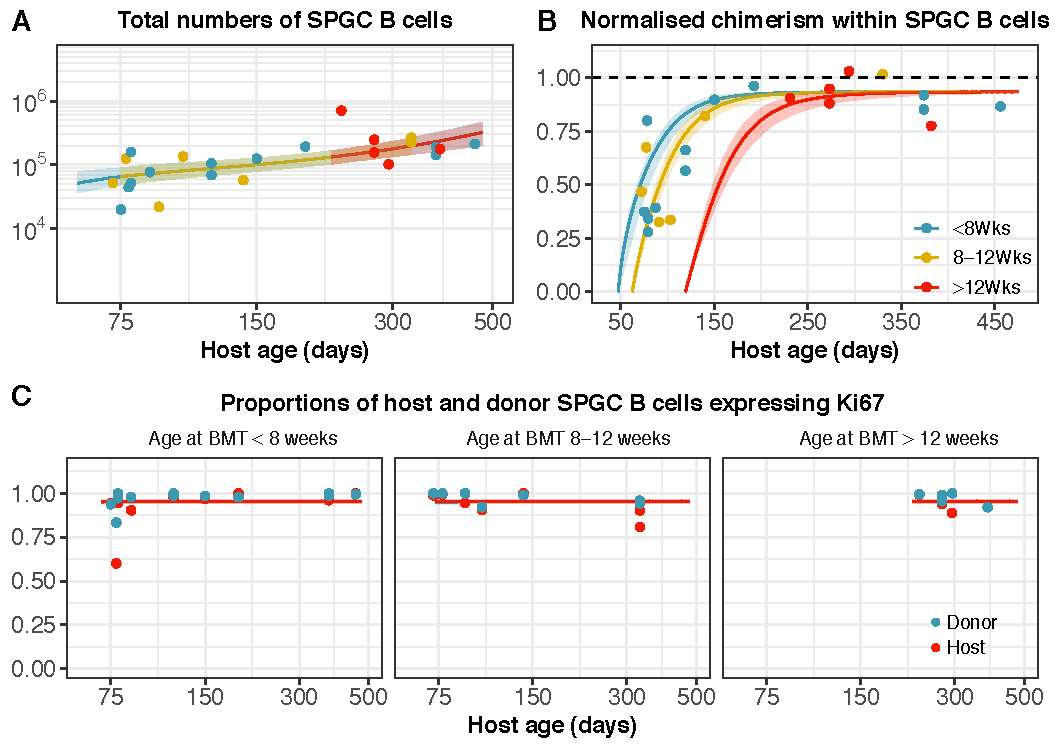
\includegraphics[scale = 0.85] {Results_SPGC_T2.pdf}}
		\caption{\textbf{Population dynamics of Spleen GC B cells in busulfan chimeric mice}, using the best-fitting model in which  cells divide at a constant rate, their mean lifespan increases with host age, and FM B cells are their precursor population. %Note that the chimerism normalised to T1 stabilises at a value <1,  equal to the chimerism in T2 normalised to T1.
Solid lines denote the  best-fitting model predictions of the  timecourses  of (A) cell counts, (B) normalised chimerism and (C)  fraction expressing Ki67. Prediction intervals (4.5$^{th}$ and 95.5$^{th}$ percentiles) were generated by drawing samples from the posterior distribution of parameter estimates. Different colours in (A) and (B) indicate mice grouped according to the age at BMT. Best-fit predictions for each group were generated using the mean age at BMT within each group.}
		\label{fig:results_SPGC}
	\end{figure}
    
    
Using this information and, as before, fitting each model simultaneously to the numbers, chimerism and Ki67 expression levels of spleen GC B cells, we found that the model of time-varying loss with T2 B cells as their immediate precursor received strongest statistical support (Table~\ref{tab:GC-AICs}; fits shown in Fig.~\ref{fig:results_SPGC}).  We find that spleen GC B cells are far more dynamic than FM B cells,  with mean lifespans and mean interdivision times of roughly half a day. The net effect of these processes yields a mean lifespan of spleen GC B cell clones of about 3 weeks in 7 week old mice (Table~\ref{tab:SPGC-parestm}). We infer that the expected lifespan of individual GC B cells doubles roughly every 5 months.
	%Models in which the rate of source influx or the inter-division time of GC cells varies with host-age produced poorer fits and received inferior statistical support  ({\looic} $\ge 8$).  
	We also infer that the maintenance of splenic GC B cell numbers is highly dependent on immigration, with approximately -- and remarkably --  35\% of the population replaced by the cells from the circulatory T2 compartment every day.
	
		%: Table GC model weights
	\begin{table}[htbp]
		\begin{center}
			\renewcommand{\arraystretch}{1.25}
			{\small
				\begin{tabular}{p{1.7cm} p{1.4cm} p{2cm} p{1.8cm} p{1.8cm} p{1.8cm} p{1.8cm} p{1.8cm}}
					\toprule
					&  & \multicolumn{6}{c}{\textbf{Model and Akaike weight (\%)}} \\
					\cline{3-8}
					                & \textbf{Source} & Simple homogeneous & Time-dependent influx & Time-dependent turnover  &  Time-dependent division &  Kinetic heterogeneity & Incumbent  \\ 
					\toprule
					Spleen GC       &   T1    &   0.0     &    0.0     &              2.0                &    1.5     &   0.0    &  0.0     \\
					                &   T2    &   0.3     &    11      & \cellcolor{blue!15} \textbf{81} &    4.1     &   0.0    &  0.1     \\
					\hline
					LN GC           &   T1    &   0.0     &   0.0      &    0.0      &    0.0     &    1                                 &    0.0    \\ 
				                    &   T2    &   0.0     &   0.0      &    0.0      &    0.0     &  \cellcolor{blue!15}  \textbf{18}    &    0.0    \\ 
				                    &   FM    &   0.0     &   0.0      &    0.0      &    0.0     &  \cellcolor{blue!15}  \textbf{81}    &    0.0    \\
				    \hline
				    \toprule
			    \end{tabular}
		    }
		\end{center}
		\caption{ \textbf{Comparison of models describing the population dynamics of Germinal center B cells in spleen and lymph nodes}. Model weights were calculated using the Leave-one-out information criterion (see Methods).} 
		\label{tab:GC-AICs}
	\end{table} 



	%The time-dependent model with T2 as the source has the fairly large probability (Akaike weight 94\%) to predict new information as compared to all the other models and sources explored in this analysis. 
	
%: Table - SP GC params
\begin{table}[htbp]
\begin{center}
		\renewcommand{\arraystretch}{1.25}
		{\small 
		\begin{tabular}{l r c}
			\toprule
			\textbf{Parameter}                                & \textbf{Estimate}   &   \textbf{95\% CI} \\
			\toprule
			\% replacement from source at  host age 7 wk (/d)            & 35                   & (21, 57)      \\
			Mean cell lifespan  at  host age 7 wk (d)                           & 0.47                 & (0.36, 0.61)  \\				
			Mean clonal lifespan at  host age 7 wk (d)                          & 22                   & (17, 28)      \\
			Mean inter-division time (d)                      & 0.48                 & (0.37, 0.63)  \\
			Time taken for $\tau$ to double (months)              & 5.2                  & (3.2, 13)      \\
			{\khi} $\rightarrow$ {\klo} transit time (d)      & 5.1                  & (3.8, 6.5)     \\					
			\hline
			\toprule 
		\end{tabular}
		}
	\end{center}
	\caption{ \textbf{Parameters governing homeostasis of GC B cells in the spleen}. Estimates from the best-fitting  model, in which the longevity of splenic GC B cells increases with host age, and T2 cells are their direct precursor.  95\% credible intervals (CI) were derived from the 2.5 and 97.5 percentiles of the posterior distributions of the parameter values.}
	\label{tab:SPGC-parestm}
\end{table} 
	
\subsection*{Lymph node GC B cells comprise a mixture of short-lived and persistent clones and derive from either T2 or FM B cells}

As in the spleen, GC B cells in lymph nodes (LN) are highly dynamic with very high levels of Ki67 expression and their numbers increasing  with age (Fig.~\ref{fig:results_LNGC}A and C). In contrast, however, donor-derived GC B cells accrued in lymph nodes relatively slowly (Fig.~\ref{fig:results_LNGC}B), suggesting that these cells turn over more slowly than splenic GC B cells, and/or are fed by their precursor population at a  lower rate.  Comparison of the alternative  models revealed strong evidence for a low rate of influx and for the existence of two subsets of LN GC B cells with rapid but distinct kinetics (Table~\ref{tab:GC-AICs}). The analysis favoured FM B cells as their direct precursor (model fits shown in Fig.~\ref{fig:results_LNGC}), with marginally lower support for a T2 precursor (Fig.~\red{SI????]}). These two models were favoured with a combined weight of $\sim$99\% relative to all other models considered (Table~\ref{tab:GC-AICs}). 

The existence of this heterogeneity, and the similarity of the kinetics deriving from the two differentiation pathways, suggests that LN GC B cells may in fact be fed by both FM and T2 cells.

% Further support for this comes from our inference that the clonal lifetimes of spleen GC B cells and the transient subset 
%We infer that one subset of LN GC B cells exhibits similar kinetics to the spleen GC B cells,  with a mean lifespan of approximately 12 hours and a comparable time between divisions, such that clones persist for several weeks. Another, more transient subset, consists of cells that are slightly longer lived but self-renew relatively slowly, such that clonal populations persist for $\sim$2 weeks on average.

\blue{THIS IS A DETAIL THAT CAN GO IN THE SI. Because we allowed for the possibility that FM B cells were the precursors to GC cells, and FM cells might form a reservoir of YFP+ cells,  the rate of loss of YFP-tagged cells provided lower bounds on the intrinsic rate of loss of each GC population.}

%: Figure - LN GC fits
    \begin{figure}[htbp]
    	\centerline{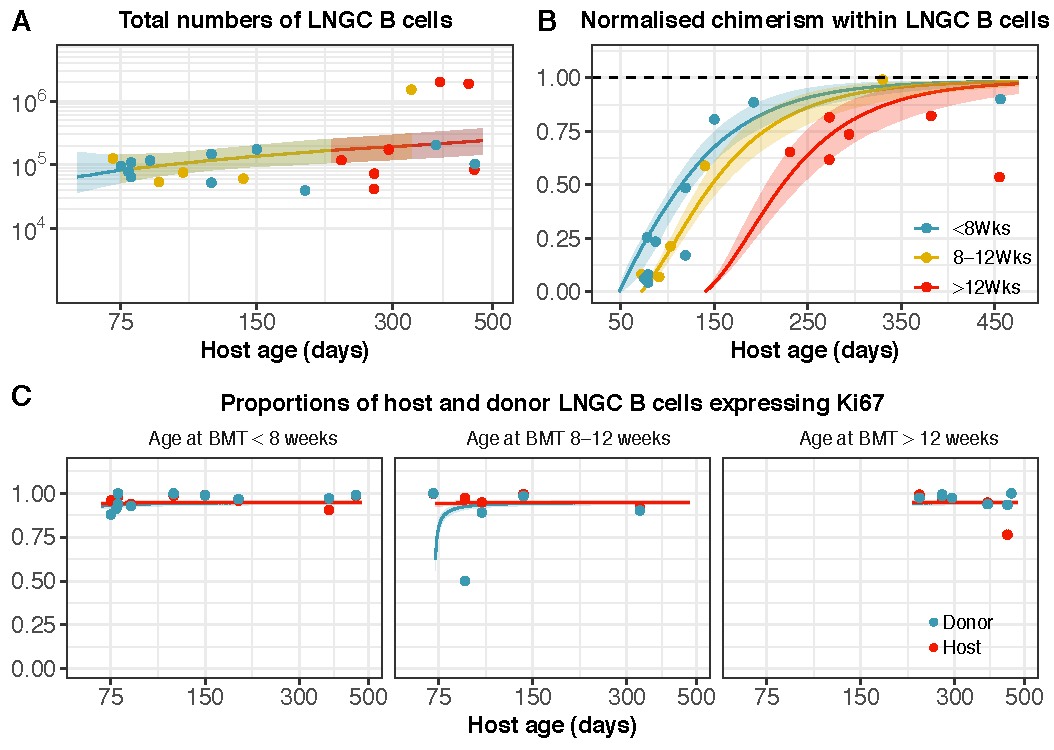
\includegraphics[scale = 0.85] {Results_LNGC_FM.pdf}}
    		\caption{ \textbf{Population dynamics of Lymph node GC B cells in busulfan chimeric mice}, using the best-fitting model in which there exist two subpopulations with different kinetics, both deriving from FM B cells.}
    		\label{fig:results_LNGC}
    \end{figure}


% GC clones are  very short-lived, with an average lifespan of $\sim$ 5 days, Table~\ref{tab:LNGC-parestm}) while others persist for on average 2 months (Table~\ref{tab:LNGC-parestm}). 

%In a 7 week old mouse, we infer that the LN GC compartment contains short and long-lived clones in roughly equal proportions. We also find that roughly 25\% of LN GC cells are replaced daily by new cells derived from the recirculating FM B cell pool.


%: Table: LN GC params with FM as the source
\begin{table}[htbp]
	\begin{center}
		\renewcommand{\arraystretch}{1.25}
		{\small
		\begin{tabular}{l r c r c}
			\toprule
			\multirow{2}{*}       \textbf{Parameter}         & \multicolumn{4}{c}{\textbf{Estimates and 95\% CI}} \\
			\cline{2-5}
			             & \multicolumn{2}{c}{\small{Transient Subset}}  & \multicolumn{2}{c}{\small{Persistent Subset}} \\
			\toprule
			\% replacement from precursors at host age 7 wk (/d)              & 0.31   & (0.01, 1.5)     & 2.6   &  (1.2, 4.7)  \\
			Mean clonal lifespan (d)                            & 13     & (8.2, 21)       & 77    &  (37, 160)  \\
			Mean inter-division time (d)                        & 2.5    & (0.65, 8.6)     & 0.55  &  (0.43, 0.73)  \\
			Mean cell lifespan  (d)                             & 1.7    & (0.63, 5.0)     & 0.54  &  (0.43, 0.72)  \\				
			Proportion of population at host age 7 wk                     & 0.75   & (0.44, 0.98)    & 0.24  &  (0.02, 0.56)    \\	
			 {\khi} $\rightarrow$ {\klo} transit time (d)       & 5.6    & (4.4, 7.1)      & 5.6   &  (4.4, 7.1)      \\	
			\hline
			\toprule 
		\end{tabular}
		}
	\end{center}
	\caption{ \textbf{Parameter estimates for LN GC B cell homeostasis}, derived from the best-fit (kinetic heterogeneity) model with FM B cells as the precursor population.  Credible intervals were estimated by taking the 2.5$^{th}$ and 97.5$^{th}$ percentiles of the posterior probability distributions of the parameters.}
	\label{tab:LNGC-parestm}
\end{table} 





\clearpage
\subsection*{Age associated  B cells linked to host and not cell age}
%Our results  indicate that FM and GC cells behave as homogenous compartments. In the case of

For both FM and GC B cell subsets we found evidence that cell lifetimes were influenced by host age. This inference is in line with studies of age associated B cells (ABCs).  ABCs are a  recently described B cell population that is specifically associated with ageing, as they are not present in substantial numbers in mice until after a year of age, after which they accumulate in number. It is not known whether this is a cell intrinsic property of ageing cells or rather influenced by host factors associated with age. To explore this, we analysed the ...




\section*{Discussion}


\section*{Methods}


\section*{Acknowledgements}
The authors acknowledge financial support from the MRC (MR/P011225/1 to BS) and the National Institutes of Health (R01 AI093870 to AY). 



\nolinenumbers % turn off line numbers before references start
% REFERENCES START HERE
% standard bst files are stored in /usr/local/texlive/2007/texmf-dist/bibtex/bst/
% my own are in~/Library/texmf/bibtex/bst/
\bibliographystyle{pnas2009} 

{\small 
\bibliography{rBcell-refs2}
}


\clearpage

%%: Table 1
%	\begin{table}[htbp]
%		\begin{center}
%			\renewcommand{\arraystretch}{1.25}
%			\begin{tabular}{c c c c c} 
%				\toprule 
%				\multicolumn{4}{c}{\textbf{Model and {\looic}}} \\
%				\cline{2-5}
%				Source &{\small Time-dependent}  & {\small Simple homogeneous} &  {\small Kinetic heterogeneity} & {\small Incumbent} \\ 
%				\toprule
%				T1    &   0             &              8             &                7              &          9         \\ 
%				T2    &   36            &              43            &                39             &          42        \\ 
%				T1 + T2 &   19          &              29            &                28             &          29        \\ 
%				\hline
%				\toprule 
%			\end{tabular}
%		\end{center}
%		\caption{\small \textbf{Comparison of models describing population dynamics of Follicular Mature (FM) B cells, pooled from LN and spleen}. Loo-ic values obtained using leave-one-out cross validation method are shown relative to that of the best fitting model, in which the rate of loss  (turnover) of FM cells declines slowly with the age of the host. Predictions of more complex models were very close to those of the simple homogenous model (that is, either very little kinetic heterogeneity, close to zero incumbent cells, or effects of cells age on turnover or division rates)}. 
%		\label{tab:FM-AICs}
%	\end{table} 
%	
	\vspace{1cm}
	
	
%	%: Table 2
%	\begin{table}[h!]
%		\begin{center}
%			\renewcommand{\arraystretch}{1.25}
%			\begin{tabular}{ l r l } 
%				\toprule 
%				\textbf{Parameter}  &  {\small Estimate}  &  {\small 95\%  $^{\ast}$CI} \\ 
%				\toprule
%				Total cell numbers at age 8.5 wks ($\times 10^{-6}$)      & 32       &  (24, 43)  \\ 
%				Percent daily replacement by source at age 8.5 wks        & 2.7      &  (2.3, 3.0)  \\
%				Mean residence time (days) at age 8.5 wks                 & 31       &  (24, 39)  \\ 
%				Mean inter-division time (days)                           & 291      &  (129, 2200)  \\
%				Time for mean residence time to double (days)             & 470      &  (270, 1400)  \\
%				Average time of loss of Ki67 expression (days)            & 6.0      &  (4.6, 7.3)  \\
%				\hline
%				\toprule 
%			\end{tabular}
%		\end{center}
%		\caption{\small \textbf{Parameter estimates from the best-fit (time-dependent) model for FM B cells (Spleen + LN)}. $^{\ast}$Credible intervals were estimated by taking 2.5$^{th}$ and 97.5$^{th}$ percentiles of the posterior probability distribution of the parameter values obtained after fitting model to the data.}
%		\label{tab:FM-parestm}
%	\end{table} 




%\begin{figure}[htbp]
%		\centerline{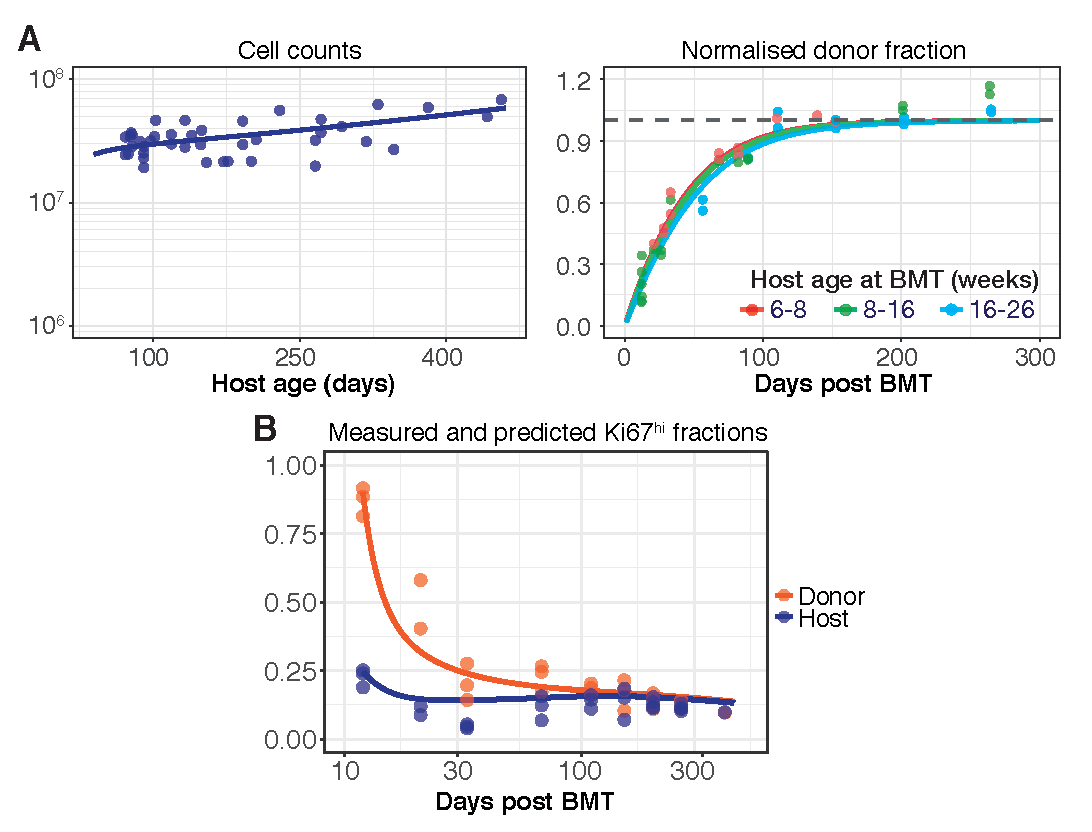
\includegraphics[scale = 0.7] {Results_FM.pdf}}
%		\caption{\small \textbf{Fitted and predicted   population dynamics of FM B cells, using the best-fitting model in which cells divide at a constant rate and their mean residence time increases with host age.}  The model was fitted simultaneously to the extended timecourses of total cell counts of FM B cells pooled from LN and spleen in busulfan chimeras, the donor fractions in FM B cells normalised to the chimerism in T1 cells and the proportion of cells that were \khi\ within host and donor FM B cells. Solid lines denote the most probable description of the observations of cell counts and normalised donor fractions and \khi fractions using the time-dependent model with purple envelopes indicating uncertainty in the model fit and the blue envelope indicates uncertainty in the data. Prediction intervals (4.5$^{th}$ and 95.5$^{th}$ percentiles) were plotted by drawing samples from the posterior distribution of parameter estimates.}
%		\label{fig:results_FM}
%\end{figure}
%


%\begin{figure}[htbp]
%	\centerline{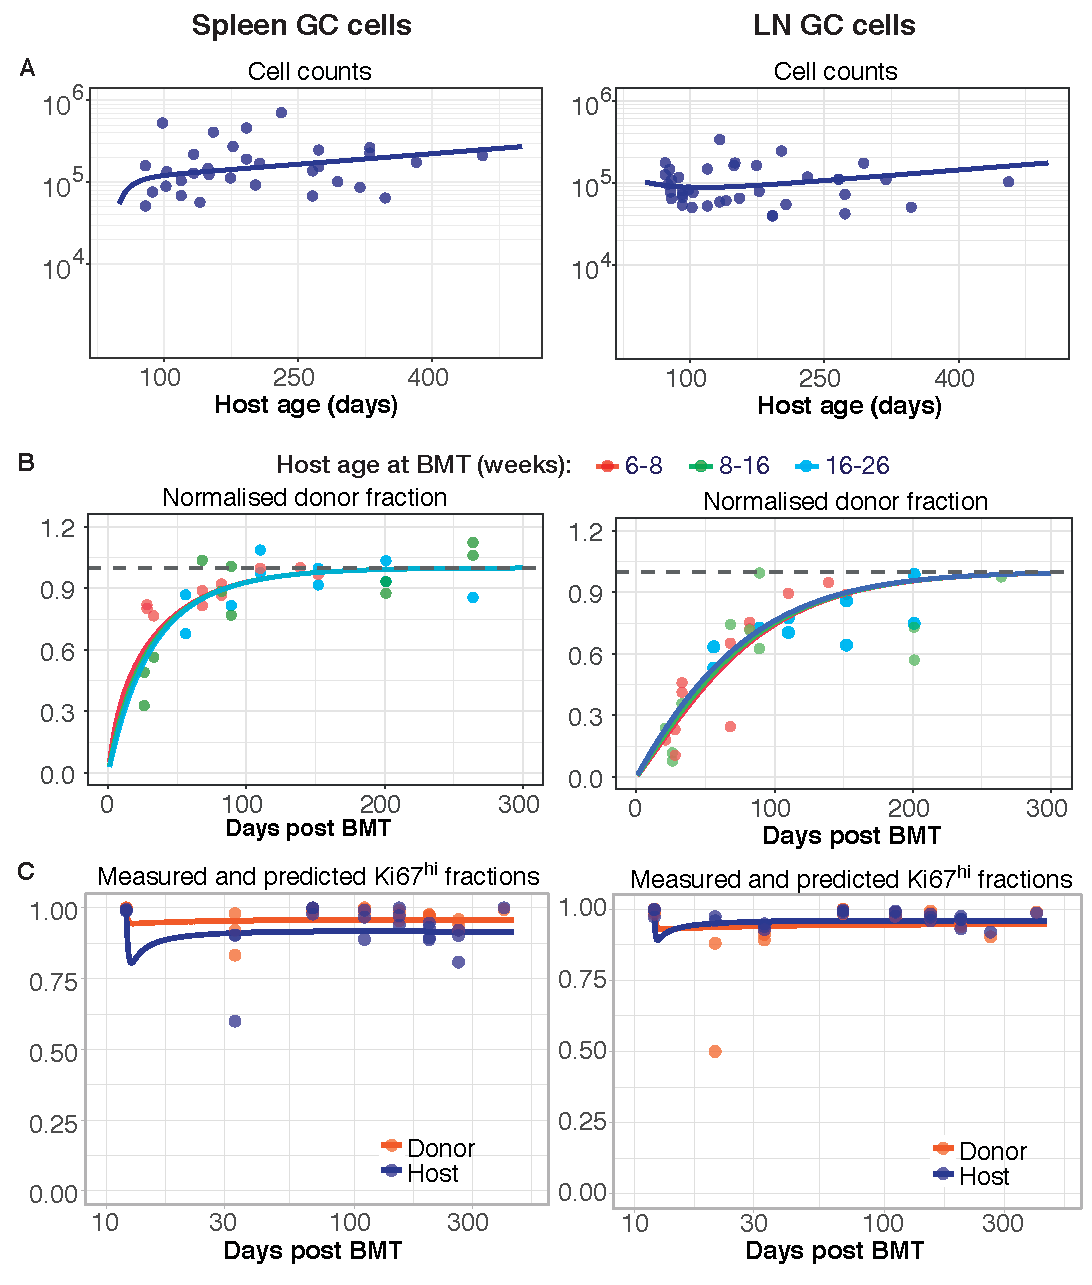
\includegraphics[scale = 0.8] {Results_GC.pdf}}
%	\caption{\small \textbf{Fitted and predicted population dynamics of spleen and LN GC B cells, using the best-fitting model in which cells the net loss rate of cells remain constant with time.}  The model was fitted simultaneously to the extended time-courses of total cell counts of spleen and LN GC B cells pooled in busulfan chimeras, the donor fractions normalised to the chimerism in FM B cells and the proportions of \khi cells within their host and donor compartments. Solid lines are the fit from the simple-homogeneous model to the observations (closed circles) of cell counts, normalised donor fractions and the proportion of cells that were \khi\ within host and donor spleen and LN GC B cells, with orange envelopes indicating uncertainty in the model while blue envelope indicate uncertainty in the data. Prediction intervals (4.5$^{th}$ and 95.5$^{th}$ percentiles) were plotted by drawing samples from the posterior distribution of parameter estimates.}
%	\label{fig:results_GC}
%\end{figure}

%: Table 1
%\begin{table}[htbp]
%	\begin{center}
%		\renewcommand{\arraystretch}{1.25}
%		\begin{tabular}{ l c c c c} 
%			\toprule 
%			& \multicolumn{4}{c}{\textbf{Model and {\looic}}} \\
%			\cline{2-5}
%			\textbf{population}  &  {\small Simple homogeneous}   & {\small Time-dependent} &  {\small Kinetic heterogeneity} & {\small Incumbent}   \\ 
%			\toprule
%			LN GC cells         & 0   &  4.9  & 1.1 & 2.9   \\ 
%			Spleen GC cells     & 0   &  0    & 0   & 1  \\ 			
%			\hline
%			\toprule 
%		\end{tabular}
%	\end{center}
%	\caption{\small \textbf{Comparison of Loo-ic values obtained using leave-one-out cross validation method are shown for different models fitted to cell counts and donor fractions in spleen and LN GC B cells normalised to the chimerism in FM cells (spleen + LN).}} 
%\label{tab:GC-AICs}
%\end{table} 
%
%%: Table 2
%\begin{table}[htbp]
%	\begin{center}
%		\renewcommand{\arraystretch}{1.25}
%		\begin{tabular}{l l r l } 
%			\toprule 
%			\textbf{Population} & \textbf{Parameter}  &  {\small Estimate}  &  {\small 95\% CI$^{\ast}$} \\ 
%			\toprule
%			\textbf{Lymph node GC cells} & Total cell numbers at age 8.5 wks ($\times 10^{-3}$)     & 62      &  (23, 188)    \\ 
%			& Percent daily replacement by source at age 8.5 wks                                    & 3.3     &  (2.8, 3.5)   \\
%			& Mean resident time (days)                                                             & 0.80    &  (0.58, 1.1)  \\ 
%			& Mean inter-division time (days)                                                       & 0.80    &  (0.59, 1.1)  \\ 	
%			& Average time of loss of Ki67 expression (days)                                        & 5.6     &  (4.2, 7.2)  \\		
%			\textbf{Splenic GC cells} & Total cell numbers at age 8.5 wks ($\times 10^{-3}$)        & 7.2     &  (1.8, 30)    \\ 
%			& Percent daily replacement by source at age 8.5 wks                                    & 57      &  (38, 97)   \\
%			& Mean resident time (days)                                                             & 0.61    &  (0.49, 0.80)  \\ 
%			& Mean inter-division time (days)                                                       & 0.60    &  (0.48, 0.79)  \\ 	
%			& Average time of loss of Ki67 expression (days)                                        & 6.2     &  (4.9, 7.7)  \\		
%			\hline
%			\toprule 
%		\end{tabular}
%	\end{center}
%	\caption{\small \textbf{Parameter estimates from the best-fit (simple homogeneous) model for spleen and LN GC B cells.}  $^{\ast}$Credible intervals were estimated by taking 2.5$^{th}$ and 97.5$^{th}$ percentiles of the posterior probability distribution of the parameter values obtained after fitting model to the data.}
%	\label{tab:GC-parestm}
%\end{table} \
%

\begin{figure}[htbp] %  figure placement: here, top, bottom, or page
   \centering
   \includegraphics[width=\linewidth]{ABCs.pdf} 
   \caption{(A) Numbers of ABCs in chimeras (B) Donor fraction amongst ABCs normalised to T1 }
   \label{fig:ABCs}
\end{figure}


\clearpage
\red{For SI ??}
%: Table: LN GC params with T2 as the source
\begin{table}[htbp]
	\begin{center}
		\renewcommand{\arraystretch}{1.25}
		{\small
			\begin{tabular}{l r c r c}
				\toprule
				\multirow{2}{*}       \textbf{Parameter}         & \multicolumn{4}{c}{\textbf{Estimates and 95\% CI}} \\
				\cline{2-5}
				& \multicolumn{2}{c}{\small{Transient Subset}}  & \multicolumn{2}{c}{\small{Persistent Subset}} \\
				\toprule
				\% replacement from source at 7wk (/d)              & 0.12   & (0.01, 0.52)    & 0.78   & (0.42, 1.3)  \\
				Mean clonal lifespan (d)                            & 13     & (8.0, 23)       & 99    &  (52, 190)  \\
				Mean inter-division time (d)                        & 2.6    & (0.71, 12)      & 0.59  &  (0.43, 0.80)  \\
				Mean cell lifespan  (d)                             & 1.6    & (0.67, 5.4)     & 0.59  &  (0.43, 0.79)  \\				
				Proportion of population at 7wk                     & 0.57   & (0.18, 0.89)    & 0.43  &  (0.11, 0.82)    \\	
				{\khi} $\rightarrow$ {\klo} transit time (d)        & 5.6    & (4.4, 7.0)      & 5.6   &  (4.4, 7.0)      \\	
				\hline
				\toprule 
			\end{tabular}
		}
	\end{center}
	\caption{ \textbf{Parameter estimates for alternative model of LN GC B cell homeostasis, sourced by T2 cells}, derived from the best-fit (kinetic heterogeneity) model.}
	\label{tab:LNGC-parestm2}
\end{table} 






\end{document}

